%%%%%%%%%%%%%%%%%%%%%%%%%%%%%%%%%%%%%%%%%%%%%%%%%%%%%%%%%%%
% Electronic Journal of Mathematics and Technology (eJMT) %
% style sheet for LaTeX.  Please do not modify sections   %
% or commands marked 'eJMT'.                              %
%                                                         %
%%%%%%%%%%%%%%%%%%%%%%%%%%%%%%%%%%%%%%%%%%%%%%%%%%%%%%%%%%%
%                                                         %
% eJMT commands                                           %
%                                                         %
\documentclass[12pt,a4paper]{article}%                    %
\usepackage{times}                                        %
\usepackage{amsfonts,amsmath,amssymb}                     %
\usepackage[a4paper]{geometry}                            %
\usepackage{fancyhdr}                                     %
\usepackage{color}                                        %
\usepackage[pdftex]{hyperref} % see note below            %
\usepackage{graphicx}%                                    %
\hypersetup{                                              %
    a4paper,                                              %
    breaklinks                                            %
}                                                         %
%                                                         %
\newtheorem{theorem}{Theorem}                             %
\newtheorem{acknowledgement}[theorem]{Acknowledgement}    %
\newtheorem{algorithm}[theorem]{Algorithm}                %
\newtheorem{axiom}[theorem]{Axiom}                        %
\newtheorem{case}[theorem]{Case}                          %
\newtheorem{claim}[theorem]{Claim}                        %
\newtheorem{conclusion}[theorem]{Conclusion}              %
\newtheorem{condition}[theorem]{Condition}                %
\newtheorem{conjecture}[theorem]{Conjecture}              %
\newtheorem{corollary}[theorem]{Corollary}                %
\newtheorem{criterion}[theorem]{Criterion}                %
\newtheorem{definition}[theorem]{Definition}              %
\newtheorem{example}[theorem]{Example}                    %
\newtheorem{exercise}[theorem]{Exercise}                  %
\newtheorem{lemma}[theorem]{Lemma}                        %
\newtheorem{notation}[theorem]{Notation}                  %
\newtheorem{problem}[theorem]{Problem}                    %
\newtheorem{proposition}[theorem]{Proposition}            %
\newtheorem{remark}[theorem]{Remark}                      %
\newtheorem{solution}[theorem]{Solution}                  %
\newtheorem{summary}[theorem]{Summary}                    %
\newenvironment{proof}[1][Proof]{\noindent\textbf{#1.} }  %
{\ \rule{0.5em}{0.5em}}                                   %
%                                                         %
% eJMT page dimensions                                    %
%                                                         %
\geometry{left=2cm,right=2cm,top=3.2cm,bottom=4cm}        %
%                                                         %
% eJMT header & footer                                    %
%                                                         %
\newcounter{ejmtFirstpage}                                %
\setcounter{ejmtFirstpage}{1}                             %
\pagestyle{empty}                                         %
\setlength{\headheight}{14pt}                             %
\geometry{left=2cm,right=2cm,top=3.2cm,bottom=4cm}        %
\pagestyle{fancyplain}                                    %
\fancyhf{}                                                %
\fancyhead[c]{\small The Electronic Journal of Mathematics%
\ and Technology, Volume 1, Number 1, ISSN 1933-2823}     %
\cfoot{%                                                  %
  \ifnum\value{ejmtFirstpage}=0%                          %
    {\vtop to\hsize{\hrule\vskip .2cm\thepage}}%          %
  \else\setcounter{ejmtFirstpage}{0}\fi%                  %
}                                                         %
%                                                         %
%%%%%%%%%%%%%%%%%%%%%%%%%%%%%%%%%%%%%%%%%%%%%%%%%%%%%%%%%%%
%
% Please place your own definitions here
%
\def\GEONExT{GEONE\kern-.06em \lower.5ex\hbox{x}\kern-.215em T}
%
%%%%%%%%%%%%%%%%%%%%%%%%%%%%%%%%%%%%%%%%%%%%%%%%%%%%%%%%%%%
%                                                         %
% How to use hyperref                                     %
% -------------------                                     %
%                                                         %
% Probably the only way you will need to use the hyperref %
% package is as follows.  To make some text, say          %
% "My Text Link", into a link to the URL                  %
% http://something.somewhere.com/mystuff, use             %
%                                                         %
% \href{http://something.somewhere.com/mystuff}{My Text Link}
%                                                         %
%%%%%%%%%%%%%%%%%%%%%%%%%%%%%%%%%%%%%%%%%%%%%%%%%%%%%%%%%%%
%
\begin{document}
%
% document title
%
\title{JSXGraph -- Dynamic Mathematics Running on (nearly) Every Device}%
%
% Single author.  Please supply at least your name,
% email address, and affiliation here.
%
\author{\begin{tabular}{c}
\textit{Michael Gerh\"auser, Bianca Valentin, Alfred Wassermann, Peter Wilfahrt} \\
alfred.wassermann@uni-bayreuth.de\\
Department of Mathematics, 
University of Bayreuth\\
95440 Bayreuth, 
Germany\end{tabular}
}%
%
%%%%%%%%%%%%%%%%%%%%%%%%%%%%%%%%%%%%%%%%%%%%%%%%%%%%%%%%%%%
%                                                         %
% eJMT commands - do not change these                     %
%                                                         %
\date{}                                                   %
\maketitle                                                %
%                                                         %
%%%%%%%%%%%%%%%%%%%%%%%%%%%%%%%%%%%%%%%%%%%%%%%%%%%%%%%%%%%
%
% abstract
%
\begin{abstract}
%
JSXGraph is a library for displaying dynamic mathematics, e.g. dynamic geometry, 
function plotting, turtle graphics, in a web browser. 
It is written in JavaScript and runs on a broad variety of devices from 
desktop computers down to smart-phones and tablet computers. 
JSXGraph is able to import various file formats like GEONEXT, GeoGebra, Intergeo, 
and---at least partially---Cinderella. 
At the moment, this seems to be the only possibility to display content from 
these sources on upcoming small computing devices, which makes them usable 
in class room.

Since Java applets seem to be on the retreat in web application, other 
approaches for displaying interactive mathematics in the web browser are needed. 
One such alternative could be our open-source project JSXGraph. It is a 
cross-browser library for displaying interactive geometry, function plotting, 
graphs, and data visualization in a web browser. It is implemented completely 
in JavaScript and uses the vector graphics formats SVG and VML. No further 
plug-ins are required.
%
\end{abstract}%
%
%%%%%%%%%%%%%%%%%%%%%%%%%%%%%%%%%%%%%%%%%%%%%%%%%%%%%%%%%%%
%                                                         %
% eJMT command                                            %
%                                                         %
\thispagestyle{fancy}                                     %
%                                                         %
%%%%%%%%%%%%%%%%%%%%%%%%%%%%%%%%%%%%%%%%%%%%%%%%%%%%%%%%%%%
%
% Please use the following to indicate sections, subsections,
% etc.  Please also use \subsubsection{...}, \paragraph{...}
% and \subparagraph{...} as necessary.
%



\section{Introduction}
In the late 1990s the availability of graphical web browsers that enabled easy access to the World Web Web 
brought many fresh ideas to the class room and to Mathematics education. 
The programming language Java became the dominant tool to raise interactivity in 
dynamic mathematics to a new level. Countless new Java-applets came to existence 
to visualize many aspects of mathematics from Kindergarten level to University level. 
Also, powerful software systems were developed that combined geometry and calculus 
under one graphical user interface. The most prominent examples are 
Cinderella~\cite{kortenkamp1999}, \GEONExT~\cite{ehmann2003} and GeoGebra~\cite{hohenwarter2005} to name a few of them.

But now a new hardware generation is on the horizon which appears to be better suited 
for the class room than the old clumsy Personal Computer. 
The revolution started with the success of small and cheap netbooks and the appearance of 
powerful smart-phones. 
Now, these two complementary worlds seem to melt together into tablet computers. 
The success of the iPad made by Apple confirms this. 
Probably, very soon many other hardware manufacturer will follow and produce 
cheaper tablet computers having more features than the iPad.

For use in class room the advantages of these devices over the Desktop PC and notebook
computers are the long battery life, their small size and weight, and their robustness.
On the other side, they offer much more possibilities than the still widely used graphical, 
programmable pocket calculators. 
These features weigh out the difficulties in using these devices---especially typing---which 
is still easier on the Desktop PC with a keyboard.

Now, mathematics education faces the challenge that most of the existing web-based software 
for dynamic mathematics is implemented in Java and embedded in web pages as so called Java applets.  
But there will be no Java plug-in available on most of these new machines. 
Without good software the new hardware is useless for learning mathematics 
in the class room.

With the project JSXGraph\footnote{\href{http://jsxgraph.org}{http://jsxgraph.org}} 
at the University of Bayreuth we try to take up 
this challenge and offer first class dynamic mathematics software that runs on 
every device including smart-phones, netbooks, tablet computers and Desktop PCs. 
Moreover, the goal is to provide compatibility for existing resources for 
mathematics education. 

JSXGraph is a free software library for mathematical visualizations in a web browser.
Its feature set covers {\sl dynamic Geometry}, plotting of {\sl function graphs}, 
{\sl curves} of various types, {\sl charts}, and {\sl turtle graphics}.

Usually, JSXGraph is embedded in web pages, for on- or off\/line viewing.
The download size is a mere 80 kByte, when embedded in web pages.
JSXGraph enhanced web pages can be viewed with all major web browsers 
on nearly every hardware platform and operating system.
The supported hardware ranges from smartphones and tablet computers 
running iOS or Android  to Desktop PC running Windows, MacOS X or Linux.

At the time of writing, JSXGraph is the only dynamic geometry system that runs  
on such a broad range of  devices and web browsers---without installation of any plug-in 
or wathsoever additional software.
JSXGraph is usable even on devices with limited computing resources, like cheap tablet computers or
older Desktop PCs running Microsoft Internet Explorer 6.0. 

Thus, this library may prove to be helpful for the
introduction of technology in mathematical education in developing countries.

JSXGraph 
is released under the Lesser GNU General Public License (LGPL), the source code
is available at Sourceforge\footnote{\href{http://sourceforge.net/projects/jsxgraph/}{http://sourceforge.net/projects/jsxgraph/}}


\section{Technical background}
The  size 
of the JSXGraph code is about 380 kByte. If the web server delivering the 
content has data compression enabled (which should be the default anyhow) the 
size of the transmitted code is about 80 kByte. To compare it with Java software, 
for example the size of the \GEONExT{} archive is about 1 Mbyte. JSXGraph does not 
rely on any other JavaScript library.

JSXGraph runs on every hardware and operating system which has a graphical 
web browser. The range of supported hardware thus reaches from Desktop PCs 
down to tablet computers and smartphones.

In order to use JSXGraph the developer has to include only two files in the 
HTML file: the JSXGraph code and a CSS file. 

JSXGraph is a pure JavaScript implementation, it does not rely on other 
libraries. JSXGraph uses the vector graphic format SVG\footnote{\href{http://www.w3.org/TR/SVG/}{http://www.w3.org/TR/SVG/}} 
for graphical output in a web browser. 
If SVG is not available, JSXGRaph falls either 
back to the alternative vector graphic format VML\footnote{\href{http://www.w3.org/TR/NOTE-VML}{http://www.w3.org/TR/NOTE-VML}} or 
to the new HTML 5 element canvas\footnote{\href{https://developer.mozilla.org/en/Canvas_tutorial}{https://developer.mozilla.org/en/Canvas\_tutorial}}.

All the mainstream web browser are supported, Firefox 3+, Internet Explorer
6+ (including the upcoming version 9), Google Chrome (all versions). 
Also, the browsers Safari, Opera are supported since at least 2008. 

For smartphones the Opera mini is supported but without interactivity.
Also Android based devices are supported since the release of the JSXGraph v0.82.
The default browser on these devices (at least up to Android 2.2) does not provide
SVG or VML graphics. But in the latest version of JSXGraph 
the use of the HTML canvas element is enabled. Thus, a new range of devices is 
able to run JSXGraph.


The widely used web browser “internet explorer” does not support SVG, but instead uses the vector graphics format VML (vector markup languag) – at least up to version number 8. The internet explorer version 9 supports SVG. Since JSXGraph is usable with SVG as well as VML, this means that JSXGraph still runs on older desktop PCs. In many cases, these outdated machines are restricted - for various reasons - to the use of  Internet Explorer 6. With  JSXGraph it is possible to access modern mathematical content even with these old machines.
Many smart-phones come with the operating system Android2, also many already announced tablet PCs are suspected to be Android based. The default web browser on Android does support neither SVG nor VML, but it allows to draw bitmap graphics with the new HTML element canvas. Starting with release 0.82, JSXGraph supports the canvas element, too. 
Even on more powerful computers JSXGraph has the advantage over Java based software that the downloading time and the initialization time is much shorter than for comparable Java-applets. 
In summary, JSXGraph is usable on a huge amount of devices and should be able to take up the challenge and support dynamic mathematics on the upcoming hardware generation.
At the time of writing, there is no other software for dynamic mathematics that can be used on such a wide range of devices.


\section{JSXGraph as DGS viewer}
JSXGraph is able to read and display the following file formats:
\begin{itemize} 
\item \GEONExT{}\footnote{\href{http://geonext.org}{http://geonext.org}} 	
	\cite{ehmann2003,ehmann2008}
\item Intergeo\footnote{\href{http://i2geo.eu}{http://i2geo.eu}} \cite{kortenkamp2009}
\item GeoGebra\footnote{\href{geogebra.org}{http://geogebra.org}} \cite{hohenwarter2005}
\item Cinderella\footnote{\href{http://cinderella.de}{http://cinderella.de}} \cite{kortenkamp1999}
\end{itemize}
The support of the \GEONExT{} file format by JSXGraph is close to 100\%. 
Only very few \GEONExT{} resources are misinterpreted by JSXGraph. 
In Figure~\ref{fig:geonext} the construction to the right is the \GEONExT{} Java-applet, to the left is the same file displayed by JSXGraph.
\begin{figure}[ht]
\begin{center}
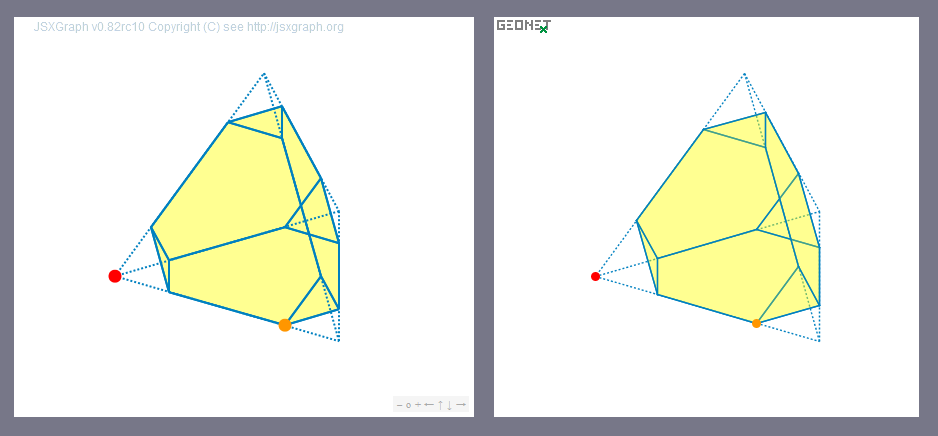
\includegraphics[width=0.8\textwidth]{geonext.png}\\
\caption{The right image shows a \GEONExT{} java applet, 
the left image contains the same construction displayed 
by JSXGraph.}\label{fig:geonext}
\end{center}
\end{figure}

The Intergeo~\cite{kortenkamp2009} format is an upcoming common file format supported by the most European implementors of dynamic geometry systems. JSXGraph possesses one of the most complete  implementiations of the file formats. At the time of writing, the file format just starts to gain popularity. 

\begin{figure}[ht]
\begin{center}
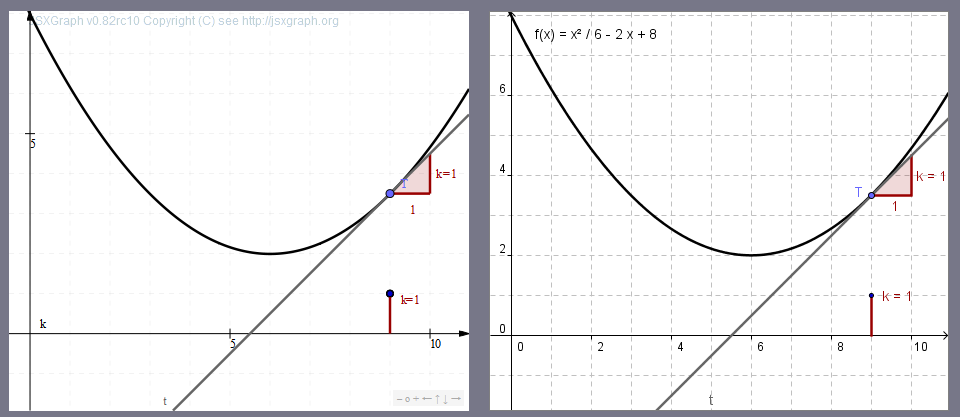
\includegraphics[width=0.8\textwidth]{geogebra.png}\\
\caption{The right image shows a GeoGebra java applet, 
the left image contains the same construction displayed 
by JSXGraph.}\label{fig:geogebra}
\end{center}
\end{figure}
The support for GeoGebra is not complete, but covers many of the most common features of  GeoGebra. In Figure \ref{fig:geogebra} the construction to the right is the GeoGebra Java-applet, to the left is the same file displayed by JSXGraph.


\begin{figure}[ht]
\begin{center}
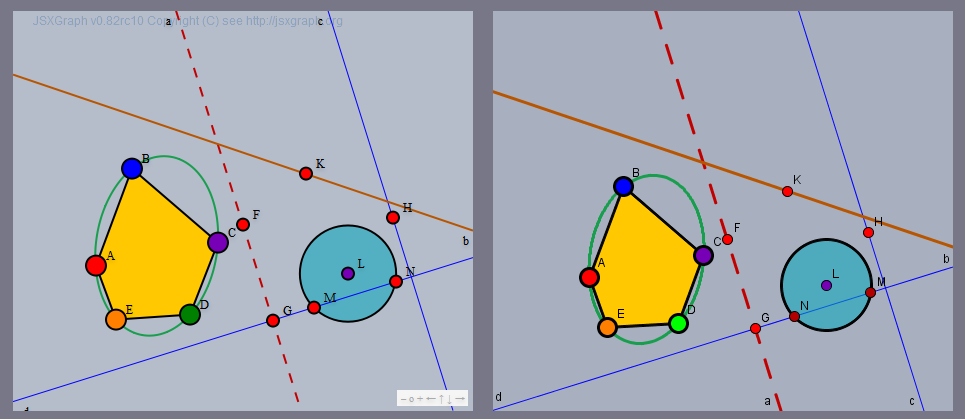
\includegraphics[width=0.8\textwidth]{cindy.png}\\
\caption{The right image shows a Cinderella java applet, 
the left image contains the same construction displayed 
by JSXGraph.}\label{fig:cindy}
\end{center}
\end{figure}
The support of the Cinderella file format \cite{kortenkamp1999} by JSXGraph is in a very early development stage. At the moment it comprises most of the Euclidean Geometry part of Cinderella. In Figure~\ref{fig:cindy} the construction to the right is the Cinderella Java-applet, to the left is the same file displayed by JSXGraph.


\section{Constructing with JessieScript}
JSXGraph comes with a simple geometric construction language called JessieScript, which is closely related to the syntax students use in school to describe their construction by compass and ruler. An example is shown in Figure~\ref{fig:jessiescript}, the online version is available at 
\href{http://jsxgraph.uni-bayreuth.de/jessie}{http://jsxgraph.uni-bayreuth.de/jessie}. 
The whole web page consists of three elements: the form for the text input of the construction, the display of the construction and a log window. 
\begin{figure}[ht]
\begin{center}
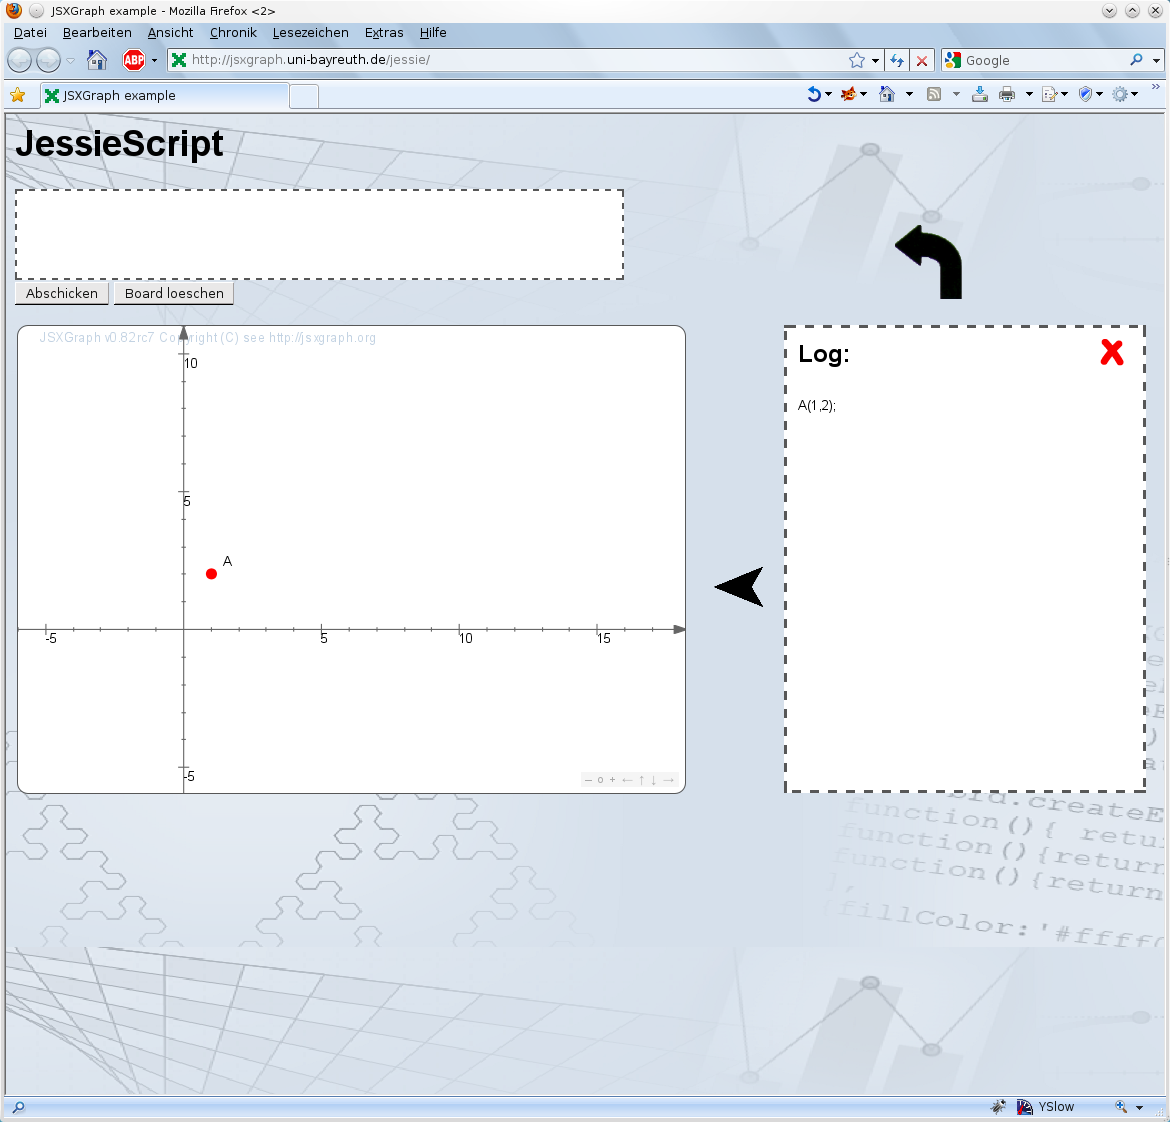
\includegraphics[width=0.8\textwidth]{jessiescript.png}\\
\caption{A simple web page for constructiong with JessieScript.}\label{fig:jessiescript}
\end{center}
\end{figure}

The most important commands are:
\begin{description}
\item{-- \verb+A(1,1)+:} Point with name '\verb|A|' at position $(1,1)$
\item{-- \verb+ZY(0.5|1)+:} Point with name '\verb|ZY|' at position $(0.5,1)$
\item{-- \verb|]AB[|:} straight line through points $A$ and $B$
\item{-- \verb|[AB[|:} ray through points $A$ and $B$, stopping at $A$
\item{-- \verb|]AB]|:} ray through points $A$ and $B$, stopping at $B$
\item{-- \verb|[AB]|:} segment through points $A$ and $B$
\item{-- \verb|g=[AB]|:} segment through points $A$ and $B$, named by '\verb|g|'
\item{-- \verb|k(A,1)|:} circle with center $A$ and radius $1$
\item{-- \verb|k(A,B)|:} circle with center $A$ through point $B$ on the circle line
\item{-- \verb|k(A,[BC])|:} circle with center $A$ and radius defined by the length of the 
(not necessarily existing) segment \verb|[BC]|
\item{-- \verb|k_1=k(A,1)|:} circle with center $A$ and radius $1$, named by '\verb|k_1|' 
\end{description}

The JSXGraph homepage contains the full description of the syntax.


\section{JSXGraph for programming Mathlets}
With JSXGraph it is possible to create special purpose mathematics visualizations.
These are sometimes called {\sl mathlets}, see for example~\cite{mitmathlets}.

JSXGraph provides an API (application programming interface) to build dynamic 
mathematics applications for the web browser. The differential equation plotter1 
on the JSXGraph home page is one example for using JSXGraph in mathematics 
education on the university level. Other applications are function plotters, 
turtle graphics, and support for various possibilities to create charts. 
This is especially interesting for publisher of e-books or provider of e-learning 
content. In this way, JSXGraph meanwhile is used in situations that are different 
from mathematics education, like medical information systems2 or landslide prediction3. 

The JSXGraph wiki4 contains more than 170 examples for dynamic mathematics, 
covering many areas like charts, function plotting, calculus, geometry, and turtle graphics, 
to name a few.

Flexible layer system.

Here is a quick overview on the available mathematical elements of JSXGraph.

\subsection{Geometry}
JSXGraph is a complete DGS (dynamic geometry system) for plane Euclidean geometry.
It contains support for homogeneous and affine coordinates. 
The following element types are available:
point, glider, intersection, circumcenter, parallel point, perpendicular point,
midpoint, mirror point, reflection point, 
line, segment, axis, tangent, normal, vector,
circle, ellipse, hyperbola, parabola, conic section,
semicircle, circumcirclearc, polygon, regular polygon, circumcircle sector,
angle, bisector, bisector lines, circum circle, perpendicular,
projective transformation.

\subsection{Calculus and function plotting}
Function plotting, parametric curves, polar plots. 
Differential equation solver.

Interpolation: Lagrange interpolation, 
cubic splines, B-splines, Bezier curves.

\subsection{Animations}


\subsection{Other topics}
Projective transformations,
Turtle graphics, 
charting.
Initial attempts to display 3D points.

\section{Exact loci computations}

\section{Other Features}
\subsection{Plug-ins}
    * moodle
    * wordpress
    * mediawiki
\begin{verbatim}
<jsxgraph width="500" height="500">
  var brd = JXG.JSXGraph.initBoard('jxgbox',{boundingbox:[-2,2,2,-2]});
  var p = brd.create('point',[1.5,1.5],{face:'o', size:8});
  brd.create('segment',[[0,0],p],{dash:3});
</jsxgraph>
\end{verbatim}                    
    * drupal 

\subsection{New features}
    * Bezier curves
    * Conic sections
    * \LaTeX{} syntax for labels and texts
          o ASCIIMathML (falls back to Google chart API)
          o MathJax (http://www.mathjax.org)
    * Animations

\subsection{Conclusion}
JSXGraph enables the usability of existing mathematical resources on a broad variety of new, small computing devices. These devices seem to be very well suited for use in class room, but up to now there is a lack of good mathematical software, since Java-applets are not longer supported. The goal of JSXGraph is to change this situation.

\begin{thebibliography}{99}
    \bibitem{crockford} Crockford D. JavaScript: The good parts, Sebastopol, CA, O'Reilly (2008).
    \bibitem{ehmann2003} Ehmann, M., Miller, C.: ``Dynamic Mathematics with \GEONExT.''
        (Part I: The Interplay between Geometry, Algebra and Calculus)
        in: T. Triandafillidis, K. Hatzikiriakou (Editors): Technology in Mathematics Teaching
        Proceedings of the 6th International Conference, University of Thessaly, Volos - Greece, October 2003, ISBN 9-60923-840-8.    
 
    \bibitem{ehmann2008} Ehmann, M., Miller, C., Wassermann, A.: ``Dynamic Mathematics with GEONExT: New Concepts''. Book of Abstracts, 4th European Workshop on Mathematical \& Scientific e-Contents
    September 2008.   

    \bibitem{hohenwarter2005} Hohenwarter, M., Fuchs, K.: ``Combination of Dynamic Geometry, Algebra and Calculus in the Software System GeoGebra''. (2005) In: Computer Algebra Systems and Dynamic Geometry Systems in Mathematics Teaching Conference 2004. Pecs, Hungary 

    \bibitem{kortenkamp2009} Kortenkamp, U., Dohrmann, Ch., Kreis, Y., Dording, C., Libbrecht, P., Mercat, Ch.: ``Intergeo - Using the Intergeo Platform for Teaching and Research''. (2009); published at ICTMT9 - The Ninth International Conference on Technology in Mathematics Teaching (FR – Metz)

    \bibitem{kortenkamp1999} Kortenkamp, U., Richter-Gebert, J.: ``Euklidische und Nicht-Euklidische Geometrie mit Cinderella''. In: Tagungsband zum N\"{u}rnberger Kolloquium zur Didaktik der Mathematik 1999.
    
    \bibitem{mitmathlets} MIT Interactive Mathematics Site {\href{http://math.mit.edu/mathlets/}{http://math.mit.edu/mathlets/}}.
    
    \bibitem{geosvg} GeometryEditor (http://wme.cs.kent.edu/geosvg/), formerly known as GeoSVG.
    
    %\bibitem http://sourceforge.net 
    %\bibitem http://i2geo.net 
    
    \bibitem{sketchpad} http://www.dynamicgeometry.com
    
    \bibitem{cabri} http://cabri.com 
    
    \bibitem{cinderella} http://cinderella.de 
    
    \bibitem{geonext} http://geonext.de 
    
    \bibitem{geogebra} http://geogebra.org
    
    \bibitem{mcallister} Neil McAllister: http://infoworld.com/d/developer-world/watch-out-java-here-comes-javascript-799
\end{thebibliography}

\end{document}